\scanpage{13}
\mspage{3}

initial form (case $\alpha,\beta$) implies Hypothesis 2 in its general form (in terms of $\alpha_0,\alpha_1,\ldots\alpha_n$).

\uline{Hypothesis} 2': For every $\alpha_0\in\mathrm{Ob}\,A$, the induced functor $A_{/\alpha_0}\unsure{\xrightarrow{\varphi}|\twoheadrightarrow|\longrightarrow}\mathcal X_{/\alpha_0}$ conforms \unsure{to|:} Hypothesis 2 i.e. for every diagram
\diagram{\begin{tikzcd}[ampersand replacement=\&,column sep=small,row sep=small]
\alpha_1\arrow[dr]\&\&\alpha_2\arrow[dl]\\
\&\alpha_0\&
\end{tikzcd}}
, considering the commutative squares in $A$ which complete it to
\diagram{\begin{tikzcd}[ampersand replacement=\&,column sep=small,row sep=small]
\&\gamma\arrow[dl]\arrow[dr]\&\\
\alpha_1\arrow[dr]\&\&\alpha_2\arrow[dl]\\
\&\alpha_0\&
\end{tikzcd}}
, i.e. the objects of $A_{/\alpha_1\times_{\alpha_0}\alpha_2}$, the family of corresponding arrows
\[U_\gamma\longrightarrow U_{\alpha_1}\times_{U_{\alpha_0}}U_{\alpha_2}\]
is covering (i.e., epimorphic).

The hypotheses Hypotheses 1, 2, 2' can be nicely reformulated, in terms of the canonical extension
\[\varphi_!:\widehat A\longrightarrow\mathcal X\]
of $\varphi$ to a functor 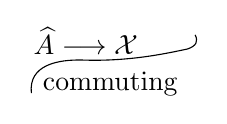
\begin{tikzpicture}[baseline=(w.base)]
\node[anchor=west,inner sep=0pt] (w) at (0,0) {commuting};
\node[anchor=west,inner sep=0pt] at (-.12,.54) {\inserted{$\widehat A\longrightarrow\mathcal X$}};
\draw (-.14,-.12)..controls(-.18,.24)and(.2,.31)..(.52,.3)..controls(1.12,.28)and(1.6,.39)..(1.84,.44)..controls(1.96,.48)and(1.98,.54)..(1.94,.62);
\end{tikzpicture} \deleted{\unsure{with|and}} with small $\lim_{\longrightarrow}$. These are respectively
\margin{12}
